\section{1174039 - Liyana Majdah Rahma}
    \subsection{Teori}
    \begin{enumerate}
        \item Jelaskan apa itu random forest, sertakan gambar ilustrasi buatan sendiri.\par
        Random forest adalah sebuah algoritma yang biasanya dipakai untuk mengklasifikasikan suatu data yang berjumlah besar. Dimana pengklasifikasiannya itu dapat menggunakan pohon yang digabungkan serta melewati training terlebih dahulu sebelum pada data sample nya. Dapat dijelaskan dari gambar dibawah bahwa klasifikasi tree ini di ambil dari data yang paling banyak.
        \begin{figure}[H]
            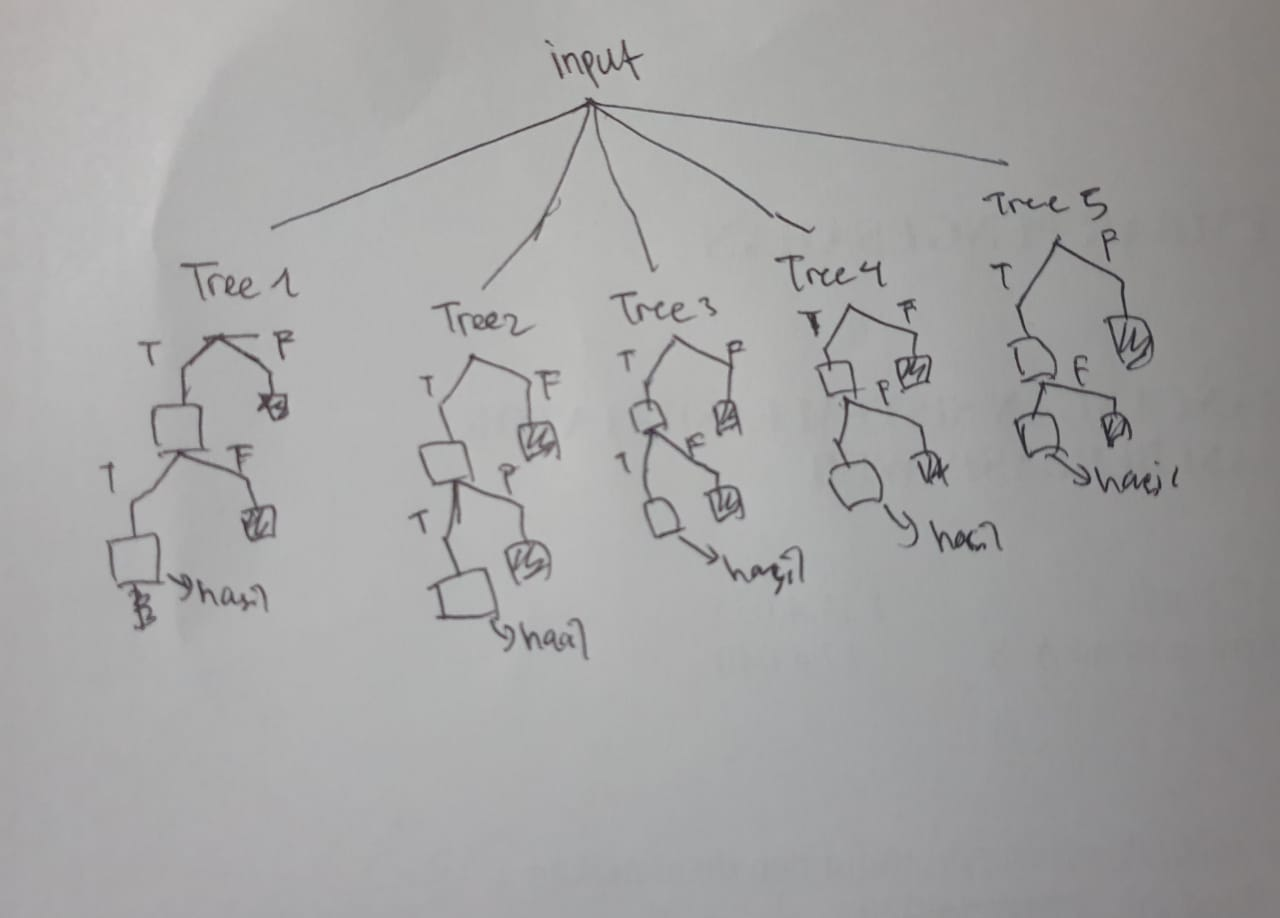
\includegraphics[width=4cm]{figures/1174039/chapter3/tree.jpeg}
            \centering
            \caption{Random Forest}
        \end{figure}

        \item Jelaskan cara membaca dataset khusus dan artikan makna setiap file dan isi field masing masing file 
\par
        langkah pertama Download terlebih dulu data yang akan dibaca, lalu buka aplikasi spyder kemudian jalankan kode nya. data yang terdapat pada file tersebut adalah data folder ATTRIBUTE, IMAGES, PARTS yang memiliki kegunaannya sendiri yang dimana pada penggunaannya data yang dipakai adalah data image\_attribute\_label pada folder attribute, data image\_class\_labels dan data classes.
        file image\_attribute\_label berguna sebagai data awal yang digunakan untuk membaca data attribute yang terdapat pada masing - masing gambar burung yang ada.
        sedangkan file image\_class\_label berguna sebagai data yang akan membuat kolom baru pada dataset yang fungsinya adalah untuk memasukan hasil dari semua data yang dimiliki oleh imgatt2.
        dan file classes berguna sebagai dataset yang akan dipanggil oleh fungsi code untuk menampilkan nama dari data burung yang dimiliki. file image\_attribute\_label
        berisi tentang data attribute yang ada pada data gambar file burung yang dimiliki difolder image pada CUB-200-2011
        file image\_class\_label
        berisi tentang data yang dimiliki oleh attribute dari image\_attribute\_label dimana data yang bernilai atau memiliki nilai disusun hingga menghasilkan data yang mudah dipahami.
        file classes
        berisi tentang data yang berguna untuk menampilkan data nama dari setiap data jenis burung yang dimiliki.

        \item Jelaskan apa itu Cross Validation. \par
        Cross Validation adalah suatu teknik yang digunakan untuk memvalidasi sebuah model serta untuk menilai pengeneralisasian dari kumpulan data independen hasil statistik analis. 
        \item Jelaskan apa arti score 44 \% pada random forest, 27 \% pada decision tree dan 29 \% dari SVM. \par
        arti score 27\% pada decission tree adalah presentasi hasil dari perhitungan dataset acak, dan arti score 29\% dari SVM adalah hasil pendekatan neural network.  Hasil tersebut didapat dari hasil valdasi silang untuk memastikan bahwa membagi training test dengan cara yang berbeda. Jadi 44\% untuk random forest, 27\% untuk pohon keputusan, dan 29\% untuk SVM. Itu merupakan presentase keakurasian prediksi yang dilakukan pada saat testing menggunakan label pada dataset yang digunakan. Score mendefinisikan aturan evaluasi model.
        \item Jelaskan bagaimana cara membaca confusion matriks dan contohnya memakai gambar atau ilustrasi sendiri. \par
        Confussion matrix menggunakan rumus perhitungan dengn 4 keluaran, yang pertama adalah :
        \begin{figure}[H]
            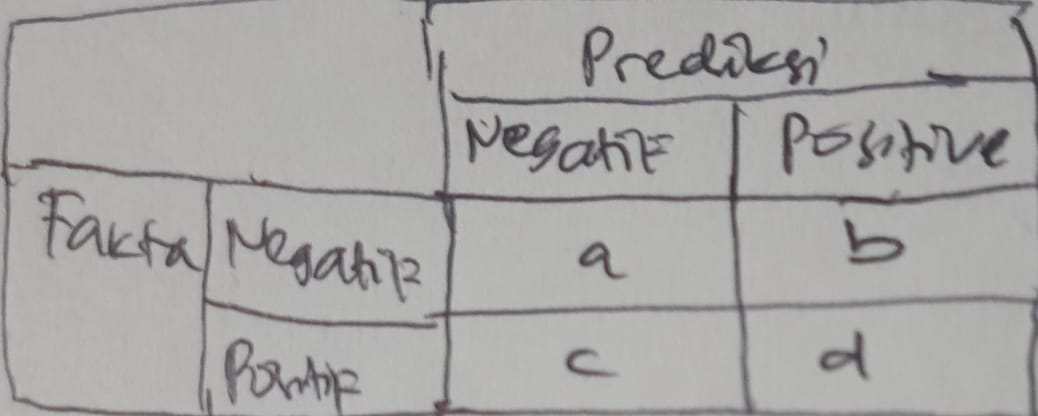
\includegraphics[width=4cm]{figures/1174039/chapter3/confusion.jpeg}
            \centering
            \caption{Confussion Matrix}
        \end{figure}
            \begin{itemize}
                \item Recall
                \begin{equation}
                    d/(c+d)
                \end{equation}
                \item Prescision
                \begin{equation}
                    d/(b+d)
                \end{equation}
                \item Accuracy
                \begin{equation}
                    (a+c)/(a+b+c+d)
                \end{equation}
                \item Error Rate
                \begin{equation}
                    (b+c)/(a+b+c+d)
                \end{equation}
            \end{itemize}
        \item Jelaskan apa itu voting pada random forest disertai dengan ilustrasi gambar sendiri. \par
        Voting itu adalah sebuah hasil dari sebuah desicion tree, yang nanti hasil  akhirnya akan menjadi hasil dari random forest. dijelaskan bahwa terdapat 5 buah tree dimana masing-masing terdapat tree satu , tree dua, tree tiga,tree empat, dan tree 5. tree satu menghasilkan A, sedangkan tree empat dan lima menghasilkan data C. Maka dapat dismpulkan data yang paling banyak diperoleh adalah data A.
        \begin{figure}[H]
            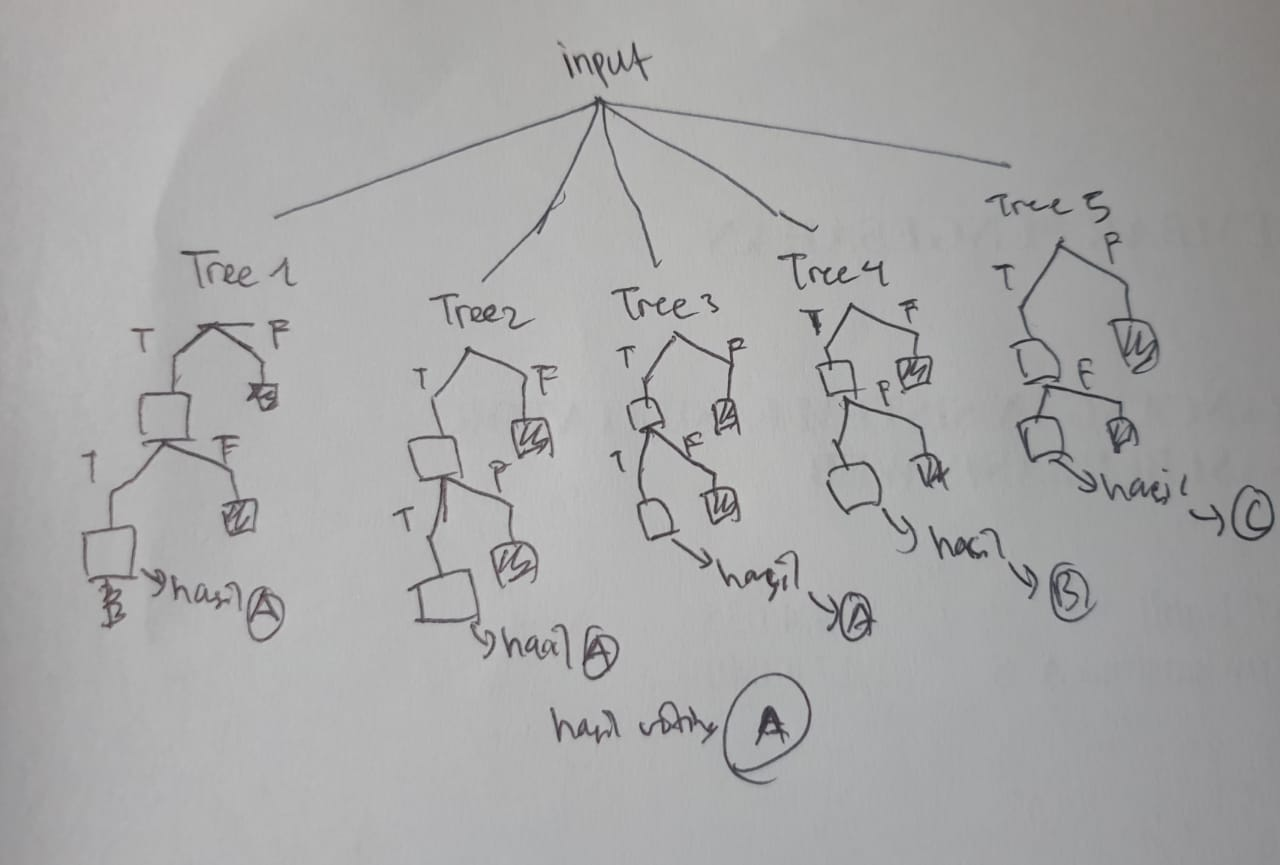
\includegraphics[width=4cm]{figures/1174039/chapter3/vote.jpeg}
            \centering
            \caption{Vote}
        \end{figure}
    \end{enumerate}
    \subsection{Praktek}
        \begin{enumerate}
            \item Pandas
            Pada baris pertama kita mengimport library pandas dan menamainya sebagai pan , lalu memasukkan data kedalam variable data. setelah itu membuat dataframe dengan data yang telah di masukkan tadi, lalu membuat variable bernama cari untuk melihat semua data dari attribute Nama lalu print variable tersebut.
            
            \begin{figure}[H]
            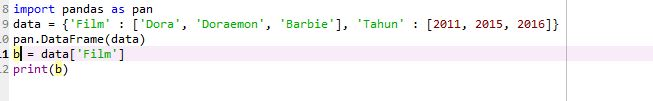
\includegraphics[width=4cm]{figures/1174039/chapter3/1.jpg}
            \centering
            \caption{Pandas}
            \end{figure}
            \begin{figure}[H]
                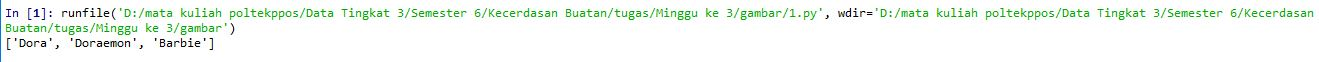
\includegraphics[width=4cm]{figures/1174039/chapter3/2.jpg}
                \centering
                \caption{hasil Pandas}
                \end{figure}
            \item numpy
            Baris pertama adalah untuk mengimport library numpy dan menamainya sebagai num, lalu membuat sebuah variable bernama mat dan menggunakan fungsi arrange untuk membuat angka berurutan dari 1 sampai 25, mengapa ditulis satu sampai 26 karena urutan dimulai dari 0,  lalu menggunakan reshape untuk mengubahnya menjadi matrix. dan terakhir print variable mat.
            \begin{figure}[H]
                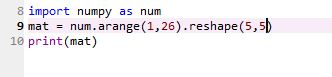
\includegraphics[width=4cm]{figures/1174039/chapter3/3.jpg}
                \centering
                \caption{Numpy}
                \end{figure}

            \begin{figure}[H]
                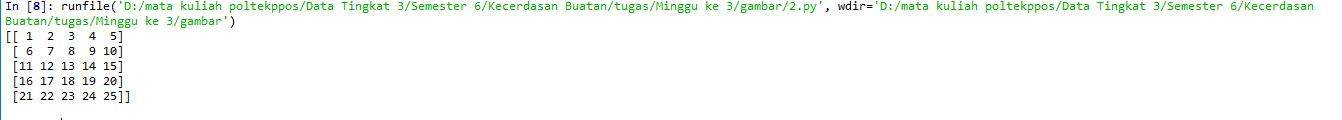
\includegraphics[width=4cm]{figures/1174039/chapter3/4.jpg}
                \centering
                \caption{Hasil Numpy}
                \end{figure}
            \item matplotlib
            Pertama import pyplot dari library matplotlib dan menamainya sebagai plt, lalu memasukkan data yang diinginkan kedalam variable x dan y . lalu menggunakan fungsi bar untuk membuat grafik bar yang isi datanya adalah x, dan y, lalu memberikan label pada sumbu x dan y dan memberikan judul pada grafik tersebut, dan menggunakan show() untuk menampilkan grafik
            \begin{figure}[H]
                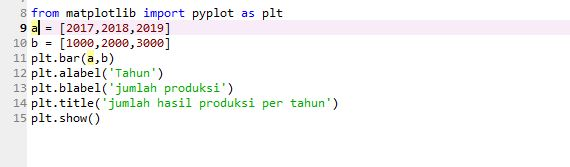
\includegraphics[width=4cm]{figures/1174039/chapter3/5.jpg}
                \centering
                \caption{Matplotlib}
                \end{figure}
            
            \begin{figure}[H]
                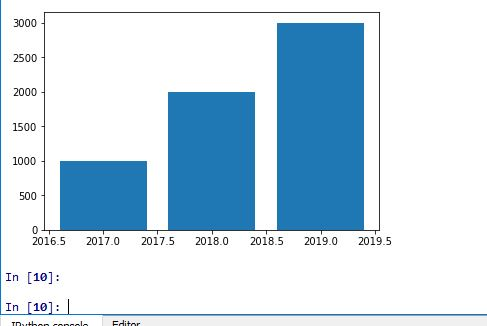
\includegraphics[width=4cm]{figures/1174039/chapter3/6.jpg}
                \centering
                \caption{Hasil Matplotlib}
                \end{figure}

            \item Random Forest
\par Dari sklearn.ensamble mengimport RandomForestClassifier dan memberikan ketentuan dimana maksimal datanya adalah 50 dengan keadaan random serta estimatornya 100 dan dimasukkan kedalam variable clf lalu itu variabel clf di running berdasarkan data training dan data label yang telah di definisikan jumlahnya. kemudian variabel clf di running berdasarkan data training paling atas untuk memunculkan hasil data training lima paling atas. setelah itu data tersebut di di running scorenya untuk melihat tingkat akurasi yang dia kerjakan maka tingkat akurasi yang dihasilkan berada pada kisaran 0,448 atau kisaran 44\%.

            \begin{figure}[H]
                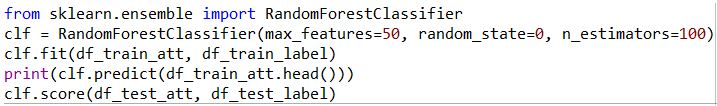
\includegraphics[width=4cm]{figures/1174039/chapter3/7.jpg}
                \centering
                \caption{Random Forest}
                \end{figure}
            \begin{figure}[H]
                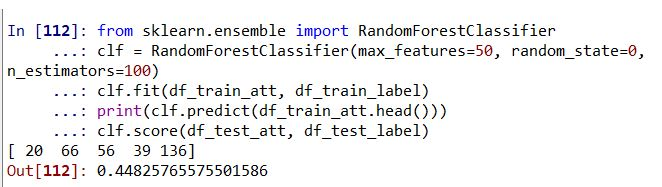
\includegraphics[width=4cm]{figures/1174039/chapter3/8.jpg}
                \centering
                \caption{Hasil Random Forest}
                \end{figure}
            \item Confussion Matrix
            dari sklearn.matrics mengimport confusion matrix  kemudian dibuat variabel pred labels dengan di isikan clf prdic df test att setelah itu membuat variabel cm yang isinya terdapat data yang di buat confusion matrix berdasarkan data test setelah variabel cm akan di running yang mana akan menghasilkan gambar berupa matrix matrix tersebut berisi nilai kebenaran yang mendekati nilai benar.
            \begin{figure}[H]
                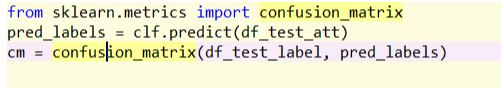
\includegraphics[width=4cm]{figures/1174039/chapter3/9.jpg}
                \centering
                \caption{Confusion Matrix}
                \end{figure}
            \begin{figure}[H]
                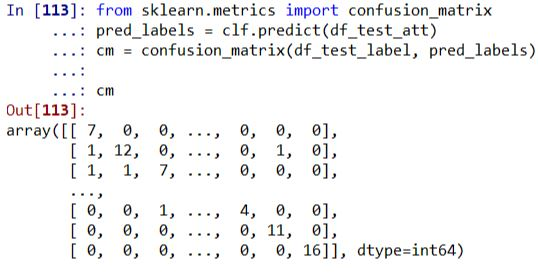
\includegraphics[width=4cm]{figures/1174039/chapter3/10.jpg}
                \centering
                \caption{Hasil Coonfusion Matrix}
                \end{figure}
            \item Decision Tree dan SVM
            masukan terlebih dahulu library tree setelah itu buat variabel clftree yang berisi decision tree setelah itu masukan nilai data training dan label yang telah di deklarasikan tadi setelah itu running variabel tersebut untuk mendapatkan score 0,266 kisaran 26 sampai 27\% akurasinya
            \begin{figure}[H]
                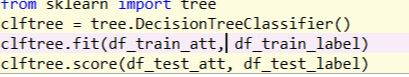
\includegraphics[width=4cm]{figures/1174039/chapter3/11.jpg}
                \centering
                \caption{Desicion Tree}
                \end{figure}
            \begin{figure}[H]
                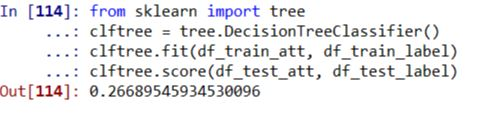
\includegraphics[width=4cm]{figures/1174039/chapter3/12.jpg}
                \centering
                \caption{Hasil Desicion Tree}
                \end{figure}
            Import terlebih dahulu library svm nya setelah itu buat variabel clfsvm yang berarti berisi nilai data training dan data label dan pendeklarasian svm itu sendiri setelah itu di running untuk mendapatkan nilai akurasinya atau score sebesar 0,283 atau dalam kisaran 23\%.
            \begin{figure}[H]
                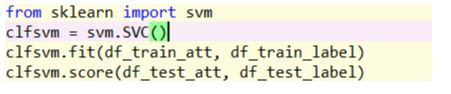
\includegraphics[width=4cm]{figures/1174039/chapter3/13.jpg}
                \centering
                \caption{SVM}
                \end{figure}
            \begin{figure}[H]
                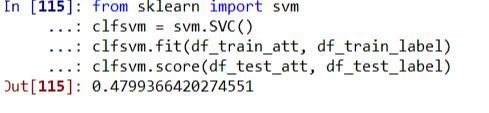
\includegraphics[width=4cm]{figures/1174039/chapter3/14.jpg}
                \centering
                \caption{Hasil SVM}
                \end{figure}
            \item Cross Validation
            mengimport cross\_val\_score dari sklearn.model\_selection , lalu memasukkan variable variable yang akan di ukur keakuratan dari model yang digunakan lalu menampilkan nya di console, disini digunakan variable clf yaitu random forest.

            \begin{figure}[H]
                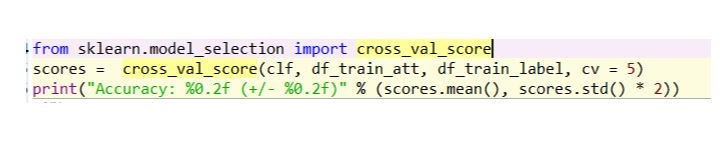
\includegraphics[width=4cm]{figures/1174039/chapter3/15.jpg}
                \centering
                \caption{Cross Val Rand Forest}
                \end{figure}
            \begin{figure}[H]
                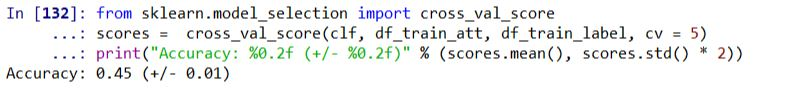
\includegraphics[width=4cm]{figures/1174039/chapter3/16.jpg}
                \centering
                \caption{Hasil Cross Validaiton Random Forest}
                \end{figure}
            
            Disini memasukkan variable variable yang akan di ukur keakuratan dari model yang digunakan lalu menampilkan nya di console, disini digunakan variable clftree yaitu desicion Tree.
            \begin{figure}[H]
                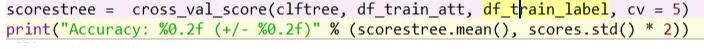
\includegraphics[width=4cm]{figures/1174039/chapter3/17.jpg}
                \centering
                \caption{Cross Vadation Desicion Tree}
                \end{figure}
            \begin{figure}[H]
                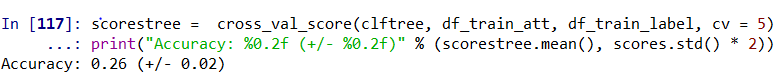
\includegraphics[width=4cm]{figures/1174039/chapter3/18.png}
                \centering
                \caption{Hasil Cross Vadation Desicion Tree}
                \end{figure}
            Disini memasukkan variable variable yang akan di ukur keakuratan dari model yang digunakan lalu menampilkan nya di console, disini digunakan variable clfsvm yaitu svm.
            \begin{figure}[H]
                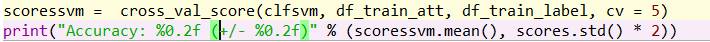
\includegraphics[width=4cm]{figures/1174039/chapter3/19.png}
                \centering
                \caption{Cross Vadation SVM}
                \end{figure}
            \begin{figure}[H]
                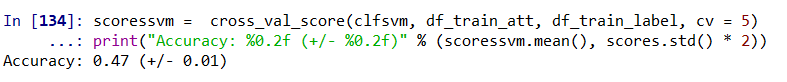
\includegraphics[width=4cm]{figures/1174039/chapter3/20.png}
                \centering
                \caption{Hasil Cross Vadation SVM}
                \end{figure}
            \item Program Pengamatan dan Hasil Pengamatan.
            perogram pengamatan ini menggunakan library matplotlib supaya hasil dari presentase hasil random forest, svm dan decision tree dapat di bandingkan dengan membuat variabel X Y Z kemudian memberikan label untuk setiap dimensinya untuk lebih jelas dapat dilihat gambar yang menunjukan hasil perbandingan presentase dari tiga metode tersebut.
            \begin{figure}[H]
                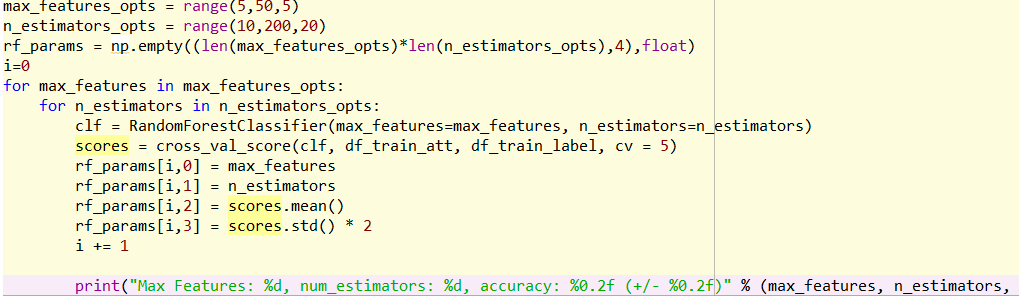
\includegraphics[width=4cm]{figures/1174039/chapter3/21.png}
                \centering
                \caption{Program Pengamatan}
                \end{figure}
            \begin{figure}[H]
                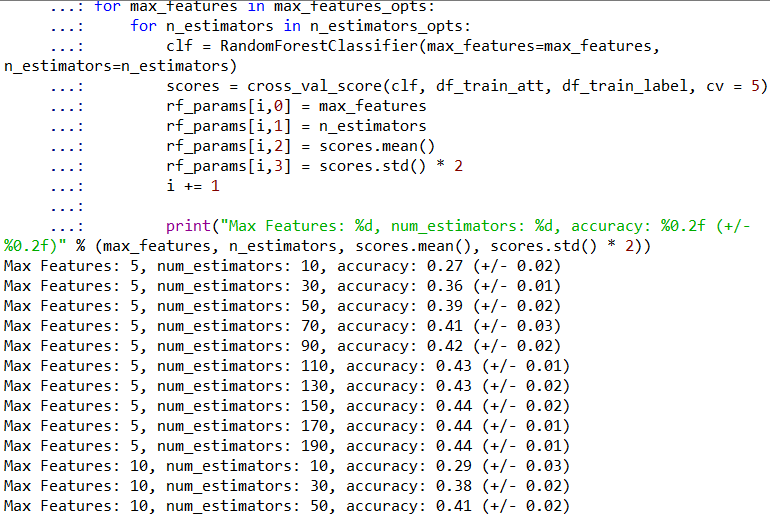
\includegraphics[width=4cm]{figures/1174039/chapter3/22.png}
                \centering
                \caption{Hasil Program Pengamatan}
                \end{figure}
            \begin{figure}[H]
                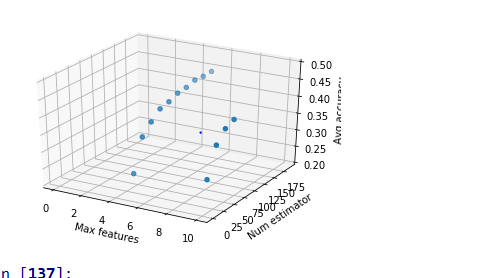
\includegraphics[width=4cm]{figures/1174039/chapter3/matplot.png}
                \centering
                \caption{Grafik Program Pengamatan}
                \end{figure}
        \end{enumerate}
    \subsection{Penanganan Error}
        \subsubsection{Skrinshoot error}
            \begin{enumerate}
                \item Error 1
                \begin{figure}[H]
                    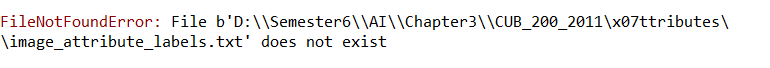
\includegraphics[width=4cm]{figures/1174039/chapter3/err1type.png}
                    \centering
                    \caption{Error 1}
                    \end{figure}
            \end{enumerate}
        \subsubsection{Kode Error dan Tipe Error}
            \begin{enumerate}
                \item Error 1 type FileNotFoundError
                \begin{figure}[H]
                    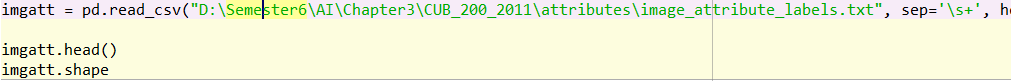
\includegraphics[width=4cm]{figures/1174039/chapter3/eror.png}
                    \centering
                    \caption{Kode Error 1}
                    \end{figure}
            \end{enumerate}
        \subsubsection{Solusi}
            \begin{enumerate}
                \item Mengganti back slash menjadi slash biasa
            \end{enumerate}